\documentclass{beamer}[10]
\usepackage{pgf}
\usepackage[danish]{babel}
\usepackage[utf8x]{inputenc}
\usepackage{beamerthemesplit}
\usepackage{graphics,epsfig, subfigure}
\usepackage{url}
\usepackage{hyperref}
\graphicspath{ {images/} }
\usepackage{parallel}
\usepackage{fixltx2e}
\usepackage{xcolor}

\definecolor{kugreen}{RGB}{0,153,153}
\setbeamercovered{transparent}
\mode<presentation>
\usetheme[numbers,totalnumber,compress,sidebarshades]{PaloAlto}
\setbeamertemplate{footline}[frame number]

  \usecolortheme[named=kugreen]{structure}
  \useinnertheme{circles}
  \usefonttheme[onlymath]{serif}
  \setbeamercovered{transparent}
  \setbeamertemplate{blocks}[rounded][shadow=true]

\logo{\includegraphics[width=0.8cm]{KULogo}}
%\useoutertheme{infolines} 
\title{A study on point in time recovery \\ on relational databases}
\author{\textbf{Author}\newline Ștefan Stan}
%\textbf{Coordonator științific} \newline Lect. dr. Cosmin-Nicolae Vârlan
\institute{
	\normalsize \textbf{Scientific Coordinator}
	\newline Lect. dr. Cristian Frăsinaru
	\newline
	\normalsize \textbf{Company Supervisor}
	\newline DevOps Engineer Gabi Ichim, TSS-Yonder
	\\
	\vspace{0.1cm}
	\small Faculty of Computer Science\\ University Alexandru Ioan Cuza from Iași}
\date{6 July 2017}

\begin{document}
\frame{\titlepage \vspace{-0.5cm}
}

\frame
{
\frametitle{Table of contents}
\tableofcontents
}

\section{Introduction}

\Large
\subsection{Keywords}

\frame{
\frametitle{Keywords}
\begin{center}
\textcolor{kugreen}{
checkpoint, recovery, point in time,\\
database, logical volume, UNIX scripts,\\
RESTful, API, cloud, Amazon Web Service}
\end{center}
}
\normalsize

\subsection{Obiectives}

\frame{
\frametitle{Obiectives}
\begin{itemize}
\item \textcolor{kugreen}{\textit{study}} the way relational databases (ex. PostgreSQL) manages transactions;
\vspace{0.3cm}
\item \textcolor{kugreen}{\textit{study}} and find a way to use PostgreSQL logging to create a management mechanism of the database changes;
\vspace{0.3cm}
\item \textcolor{kugreen}{\textit{create}} a tool that enables a user to restore a database instance state to one in a specific point in time;
\vspace{0.3cm}
\item \textcolor{kugreen}{\textit{investigate}} the possibilities and find a solution to \textcolor{kugreen}{\textit{facilitate}} usage of previously created tool to persons without UNIX/ PostgreSQL specific knowledge.
\end{itemize}
}

\section{Studies}

\subsection{Point in time recovery}
\frame{
\frametitle{Studies - Point in time recovery}
\hspace{0.5cm}\textcolor{kugreen}{Basebackup}\\
\hspace{1cm} - checkpoint from which it can be started the point in time recovery\\
\vspace{0.3cm}
\hspace{0.5cm}\textcolor{kugreen}{Write Ahead Logs (WALs)}\\
\hspace{1cm} - binary sequences that PostgreSQL generates to keep its logging (information about transactions)\\
\vspace{0.3cm}
\hspace{0.5cm}\textcolor{kugreen}{Point in time recovery (PITR)}\\
\hspace{1cm} - the process of changing a database current state to one at a specific point in time, given as input.\\
}

\subsection{Logical Volumes Management}
\frame{
\frametitle{Studies - Logical Volumes Management (LVM)}
\hspace{0.5cm}\textcolor{kugreen}{Advantages:}\\
\hspace{1cm} - flexible "disks" called logical volumes (no longer depend on physical space of harddisks )\\
\hspace{1cm} - abstraction layer above storage units\\
\vspace{0.3cm}
\hspace{0.5cm}\textcolor{kugreen}{Physical volume (PV)} - a partition with LVM metadata asociated.\\
\hspace{0.5cm}\textcolor{kugreen}{Volume Group (VG)} - a way of organizing physical volumes to enable subdivisions and their management.\\
\hspace{0.5cm}\textcolor{kugreen}{Logical Volume (LV)} - a subdivision of a volume group, which may has its space allocated from different physical volumes.\\
}

\section{Implementation}

\subsection{Logical volumes architecture}

\frame{
\frametitle{Implementation - Logical volumes architecture}
\begin{figure}[h]
	\centering
    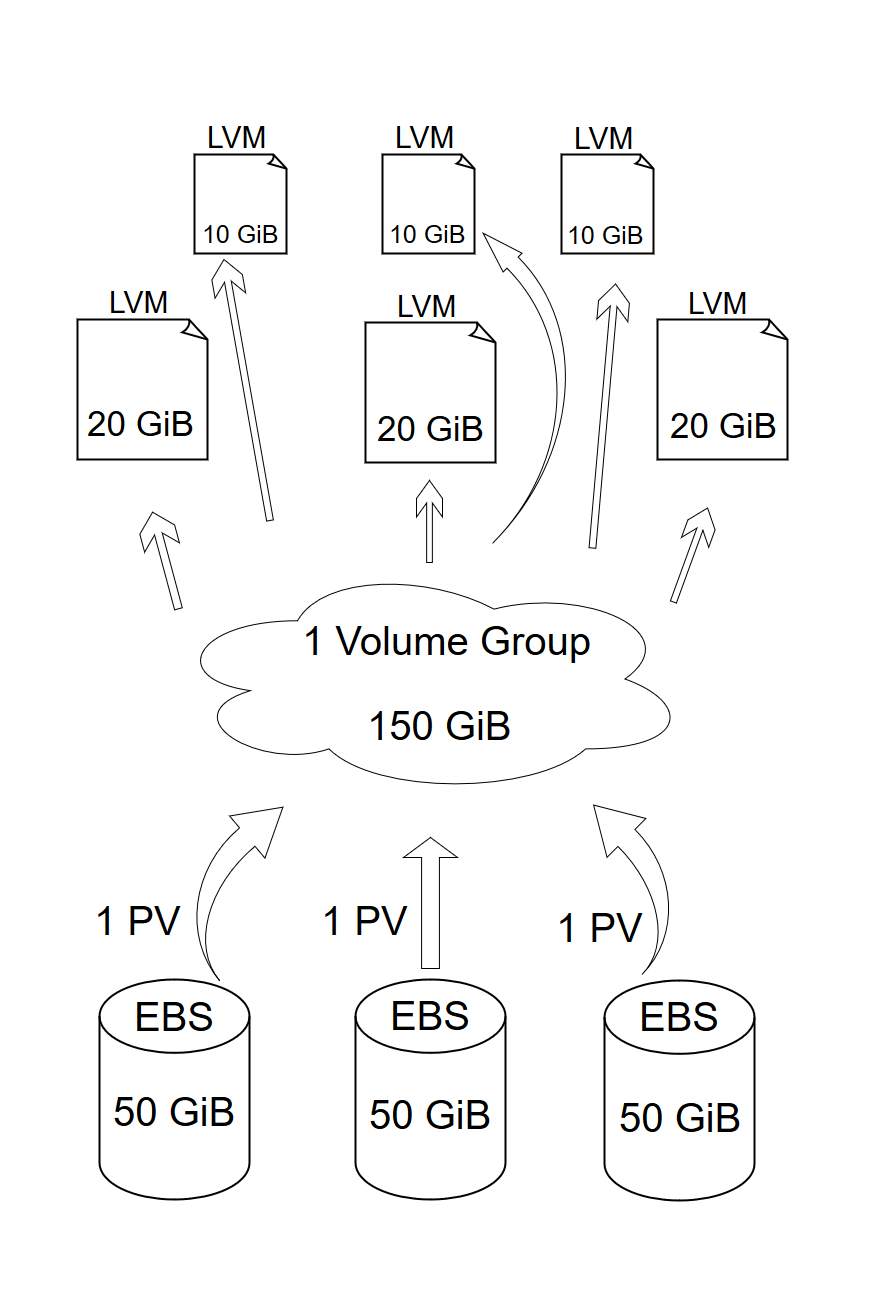
\includegraphics[scale=0.23]{LVM}
\end{figure}
}

\subsection{System architecture}

\frame{
\frametitle{Implementation - System architecture}
\begin{figure}[h]
	\centering
    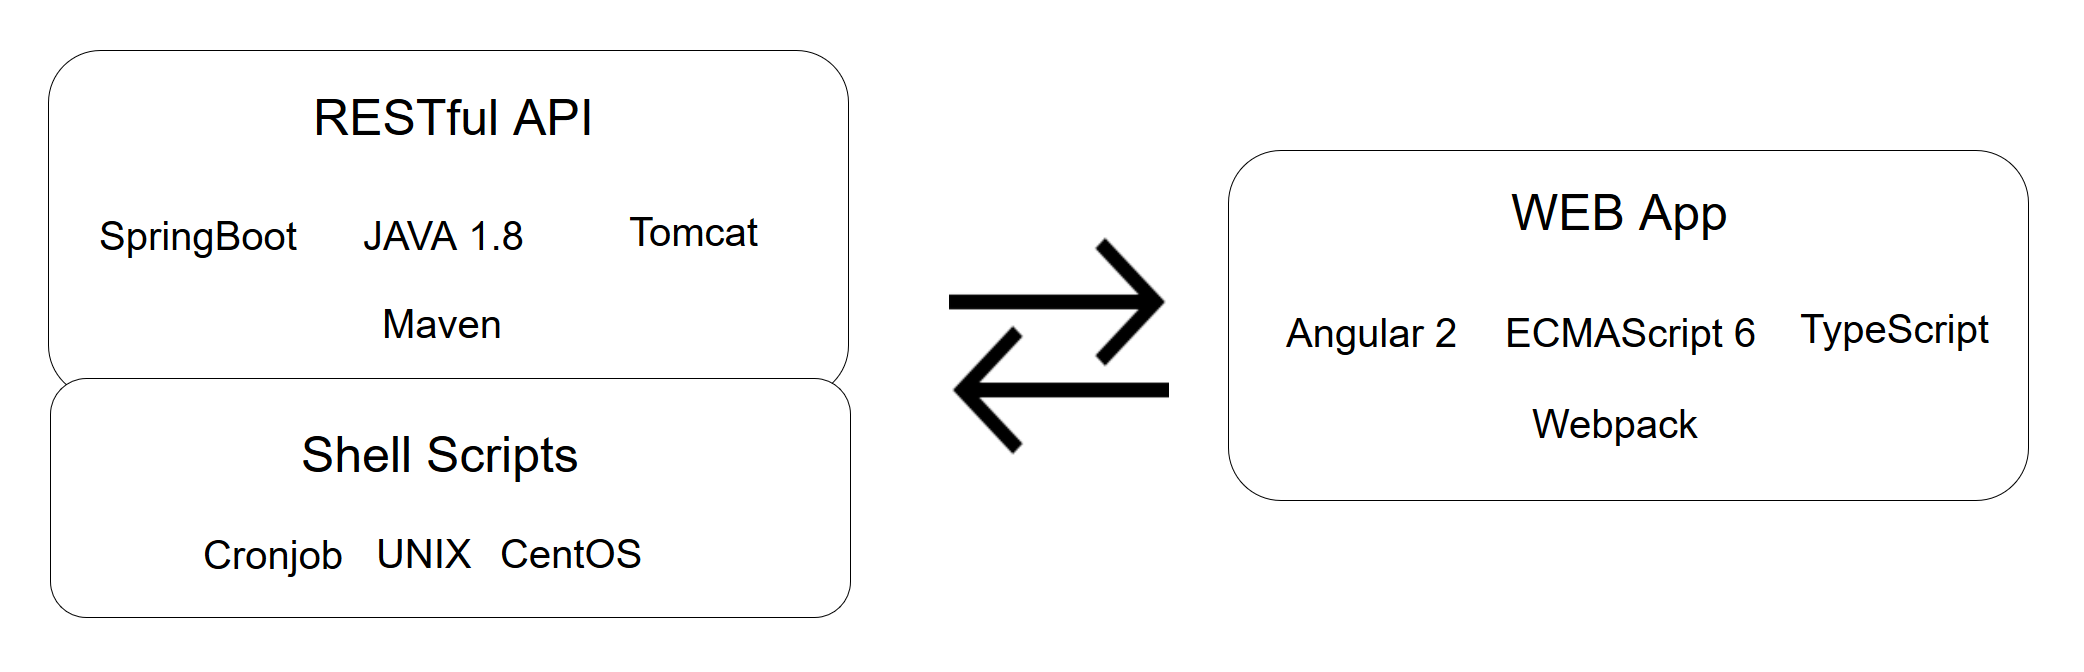
\includegraphics[scale=0.195]{LayeredArchLandscape}
\end{figure}
}

\frame{
\frametitle{Deployment - Amazon Web Services (AWS)}
\hspace{0.5cm}\textcolor{kugreen}{Advantages:}\\
\vspace{0.1cm}
\hspace{1cm} - simulate a production environment;\\
\vspace{0.1cm}
\hspace{1cm} - physical volumes used in LVM architecture are provided by EBS (Elastic Block Storage) service which guarantees data guarantees availability in case of disaster by using replication in 3 different data centers;\\
\vspace{0.1cm}
\hspace{1cm} - IaaS (Infrastructure as a service) access, which is needed to setup LVM architecture.\\
\vspace{0.1cm}
\hspace{0.5cm}\textcolor{kugreen}{Disadvantages:}\\
\vspace{0.1cm}
\hspace{1cm} - AWS costs.\\
}

\section{Use Cases}
\frame{
\frametitle{Use Cases}
\begin{itemize}
\item The worst has happened, \textcolor{kugreen}{databased crushed/stopped} and after restarting it has \textcolor{kugreen}{inconsistent data}. The tool build can be used from its web interface to \textcolor{kugreen}{restore} the database to a consistent state at a \textcolor{kugreen}{specified time};
\vspace{0.1cm}
\item A tester wants to run a suite of test cases which will\\\textcolor{kugreen}{alter the data} in some way. It realises that what he did was wrong and he wants to \textcolor{kugreen}{restore} the database in the\\\textcolor{kugreen}{exact state} it was \textcolor{kugreen}{at a specified time}.\\He has \textcolor{kugreen}{no knowledge} of SQL or Unix. 
\end{itemize}
}

\section{Future dev}
\frame{
\frametitle{Future development directions}
\begin{itemize}
\item study different databases also\\(right now works only with PostgreSQL);
\vspace{0.1cm}
\item offer an abstraction layer over different databases;
\vspace{0.1cm}
\item improve web design, refactor Angular components and also HTML and CSS
\end{itemize}
}

\section{Conclusions}

\frame{
\frametitle{Conclusions}
\begin{itemize}
\item \textcolor{kugreen}{studied} and understood the way PostgreSQL manages database changes;
\item \textcolor{kugreen}{studied} and understood how to use LVM to combine database point in time recovery with "flexible" UNIX partitions to minimize downtime of the database;
\item \textcolor{kugreen}{build} an app which facilitates restoring of PostgreSQL databases at a given time, and management (start/ stop/ status queries);
\item \textcolor{kugreen}{deployed and tested} the created solution on a\\similar \textcolor{kugreen}{production} cloud \textcolor{kugreen}{Amazon Web Services} (AWS) environment.
\end{itemize}
}

\section{Bibliography}
\frame{
\frametitle{Bibliography}
\begin{thebibliography}{7}
\footnotesize

\bibitem{RHEL}
\newblock Sander van Vugt,
\newblock Red Hat® RHCSA™/RHCE® 7 Cert Guide: Red Hat Enterprise Linux 7 (EX200 and EX300)

\bibitem{PITR}
\newblock Postgres Documentation
\newblock https://www.postgresql.org/docs/9.5/static/continuous-archiving.html

\bibitem{GOF}
\newblock E.~Gamma, R.~Helm, R.~Johnson, and J.~Vlissides.
\newblock Design Patterns: Elements of Reusable Object-Oriented Software. Addison-Wesley, 2005.

\bibitem{SPRING}
\newblock {Craig Walls},
\newblock Spring in Action, Third Edition

\end{thebibliography}
}

\end{document}
